\documentclass[8pt,unicode]{beamer}
\usetheme{ttiposter}

% geometries

\geometry{paper=a4paper,landscape}

% packages

\usepackage{luatexja}
\usepackage{amsmath}
\usepackage{graphicx}
\usepackage[labelformat=empty]{caption}
\usepackage{subcaption}
\captionsetup{compatibility=false}
\usepackage{setspace}
\AtBeginDocument{% HACKING
  \addtolength\abovedisplayskip{-2\baselineskip}
  \addtolength\belowdisplayskip{0\baselineskip}
}

% miscellaneous commands

%\definecolor{tenjugreen}{rgb}{0.4,0.8,0.4}
\newcommand{\columnscale}{0.32}
\newcommand{\tablefontsize}{\small}
\newcommand{\itemtitle}[1]{\textbf{#1} \\}
\newcommand{\arrow}{{\color{ttiblue} →}\hspace{1ex}}
\newcommand{\good}[1]{\textbf{\color{orange} #1}}
\newcommand{\bad}[1]{\textbf{\color{blue} #1}}
\newcommand{\keyword}[1]{\textbf{\color{red} #1}}

% title setting

\title{カテゴリ間の関連性を利用した多層ニューラルネットワークによる文書分類}
\author{外山洋太 三輪誠 佐々木裕}
\institute{豊田工業大学 工学部 先端工学基礎学科}
\date{2015/9/4}


\begin{document}
\begin{frame}{}
\vspace{-8ex}
\begin{columns}[t]

\begin{column}{\columnscale\textwidth} % first
  \begin{block}{背景と目的}
    \begin{itemize}
      \item \itemtitle{タスク}
        文書を複数のカテゴリについて多値分類
        \begin{itemize}
          \item カテゴリ:ラベルが付けられる各項目
          \item 従来の手法では...
            \begin{itemize}
              \item カテゴリ同士の関連性を\bad{手動で変化}させ考慮
              \item 文書の数値表現であるBoWは文書内の\bad{語順を無視}
            \end{itemize}
        \end{itemize}
      \item \itemtitle{目的}
        \begin{itemize}
          \item \keyword{多層ニューラルネットワーク}によりカテゴリ間の関連性を
            \good{自動的に}考慮 \\
          \item \keyword{パラグラフベクトル}の使用により
            \good{語順や単語の位置関係を考慮}
        \end{itemize}
    \end{itemize}
  \end{block}

  \vspace{-1em} % HACKING
  \begin{figure}
    \caption{例. カテゴリ毎のラベルが付いた文書(商品レビュー)}
    \begin{subfigure}{0.52\textwidth}
      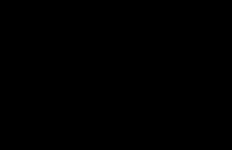
\includegraphics[width=\textwidth]{fig/reviewcomment.png}
    \end{subfigure}
    \begin{subfigure}{0.32\textwidth}
      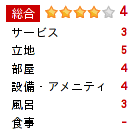
\includegraphics[width=\textwidth]{fig/reviewpoints.png}
    \end{subfigure}
  \end{figure}

  \begin{block}{関連研究}
    \begin{itemize}
      \item \itemtitle{隠れ状態を用いたホテルレビューのレーティング予測 [1]}
        文書内の各文に対して推定した隠れレーティングと
        レビュー全体のレーティングとの\bad{繋がりを手動で変化}させる \\
        \arrow カテゴリ間の関連性を考慮
      \item \itemtitle{パラグラフベクトル [2]}
        \good{語順を考慮}した文書の数値表現。
        文書分類に有用であることが実験により示されている。
      \item \itemtitle{vLBL+vLBL(c) [3]}
        \good{単語同士の位置関係を考慮}した単語ベクトルの学習手法。
        パラグラフベクトルまたは文ベクトルも同時に学習可能。
    \end{itemize}
  \end{block}

  \begin{block}{提案手法}
    \begin{itemize}
      \item \keyword{パラグラフベクトル}に加え\keyword{文ベクトル}を導入した
        \keyword{vLBL+vLBL(c)}を提案
        \good{語順と単語同士の位置関係を考慮}した文書の数値表現を生成 \\
        \arrow 文書の意味をより正確に表現
      \item 分類器としての\keyword{多層ニューラルネットワーク} \\
        \arrow カテゴリ間の関連性を\good{自動的に考慮}
    \end{itemize}
  \end{block}
\end{column} % first

\begin{column}{\columnscale\textwidth} % second
    \begin{figure}
      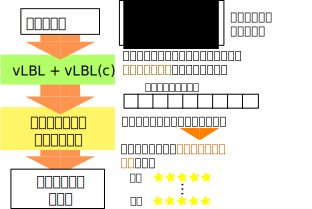
\includegraphics{fig/architecture.png}
      \caption{文書データからのカテゴリ毎のラベル推定}
      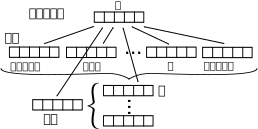
\includegraphics{fig/vectors.png}
      \caption{\keyword{vLBL+vLBL(c)}による単語及び文、文章ベクトルの学習}
    \end{figure}

    {\Large
    \begin{gather*}
      g = \sum_t \left\{ \log\sigma(s(t))
          + \sum^K_{t' \sim P_n} \log(1 - \sigma(s(t'))) \right\} \\
      s(t) = {\bf c}_t \cdot {\bf w}_t
             + {\bf c}^{loc}_t \cdot {\bf w}^{loc}_t + b_t \\
    \end{gather*}
    }
    \begin{gather*}
      \left(
      \begin{matrix}
        t : 現在の単語の位置 \\
        c_t, w_t : 文脈、単語を表すベクトル \\
        s : 位置関係を考慮した単語と文脈の類似度 \\
        σ : シグモイド関数
      \end{matrix}
      \right)
    \end{gather*}

    \begin{itemize}
      \item 現在の単語\(w_t\) \arrow 文脈との意味を近く
      \item 文脈外の単語\(w_{t'}\) \arrow 文脈との意味を遠く
      \item \({\bf c}^{loc}_t \cdot {\bf w}^{loc}_t\)の項により単語同士の
        位置関係を考慮
    \end{itemize}
\end{column} % second

\begin{column}{\columnscale\textwidth} % third
  \begin{block}{予備実験}
    vLBL+vLBL(c)とSVMまたは多層NNを用い、
    従来の手法[1]と同じ多値分類問題の精度を測定

    \begin{itemize}
      \item \itemtitle{目的}
      \begin{itemize}
        \item パラグラフベクトルの有効性の調査
        \item 従来手法との比較による目標設定
      \end{itemize}

      \item \itemtitle{実験設定}
      \begin{itemize}
        \item 宿泊予約サイト楽天トラベルのホテルレビューデータを利用
        \item 入力データは、各レビューのコメント部分と7カテゴリのレーティングの
        組(各カテゴリのレーティングは評価なしを含む6段階評価)
        \item 訓練データ:300,000件、評価データ:10,000件
        \item 多層NNの入力は位置を考慮した及び考慮していない
        2つのパラグラフベクトル
      \end{itemize}

      \item \itemtitle{結果及び考察}
        より表現力の高い文書の数値表現の評価や、多層NNのパラメータ最適化が必要

      %\begin{table}
      %  \small
      %  \caption{\small 点数推定プログラムのパラメータ設定}
      %  \begin{tabular}{l | r}
      %    項目 & 値 \\
      %    \hline
      %    学習する単語の範囲 & 前後5単語 \\
      %    単語の最少出現回数 & 5回 \\
      %    ベクトルの次元数 & 400 \\
      %    中間層の数 & 1 \\
      %    入力層でのニューロン数 & 800個 \\
      %    中間層でのニューロン数 & 200個
      %  \end{tabular}
      %\end{table}

      %\begin{figure}
      %  \includegraphics[width=0.6\textwidth]{fig/result.png}
      %  \caption{各手法における点数推定精度}
      %\end{figure}
    \end{itemize}

    \vspace{-1em} % HACKING
    \begin{figure}
      \centering
      \begin{minipage}[t]{0.45\textwidth}
        \centering
        \small
        \caption{\small プログラムのパラメータ設定}
        \begin{tabular}{l | r}
          項目 & 値 \\
          \hline
          学習する単語の範囲 & 前後5単語 \\
          単語の最少出現回数 & 5回 \\
          ベクトルの次元数 & 400 \\
          中間層の数 & 1 \\
          入力層でのニューロン数 & 800個 \\
          中間層でのニューロン数 & 200個
        \end{tabular}
      \end{minipage}\hfill
      \begin{minipage}[t]{0.45\textwidth}
        \centering
        \vspace{0em}
        \includegraphics[width=\textwidth]{fig/result.png}
        \caption{\small 各手法における点数推定精度}
      \end{minipage}
      %\begin{minipage}[t]{0.45\textwidth}
      %  \centering
      %  \small
      %  \vspace{0em}
      %  \caption{\small 各手法における点数推定精度}
      %  \begin{tabular}{l | r}
      %    項目 & 精度(\%) \\
      %    \hline
      %    実験手法(SVM)& 33.6 \\
      %    実験手法(多層NN)& 37.7 \\
      %    従来の手法[1] & 48.3
      %  \end{tabular}
      %\end{minipage}
    \end{figure}
  \end{block} % 実験

  \begin{block}{まとめと今後の課題}
    \begin{itemize}
      \item パラグラフベクトルと多層ニューラルネットワークとを
        組み合わせただけでは精度が不十分
      \item 課題
        \begin{itemize}
          \item vLBL+vLBL(c)における文ベクトルの評価
          \item 多層ニューラルネットワークのパラメータ最適化
          \item 提案手法の有用性の評価
        \end{itemize}
    \end{itemize}
  \end{block} % まとめ

  参考文献 \\
  \begin{enumerate}
  \item 藤谷宣典ら, 隠れ状態を用いたホテルレビューのレーティング予測.
  言語処理学会 第21回年次大会, 2015. \\
  \item Quoc Le et al., Distributed Representations of Sentences and Documents.
  ICML 2014, 2014. \\
  \item 森洸樹ら, 英文穴埋め問題における文章ベクトルと学習データの質の影響.
  第222回自然言語処理研究会, 2015.
  \end{enumerate}
\end{column} % third

\end{columns}
\end{frame}
\end{document}
